%%%%%%%%%%%%
%
% $Autor: Wings $
% $Datum: 2019-03-05 08:03:15Z $
% $Pfad: TemplateSensor $
% $Version: 4250 $
% !TeX spellcheck = en_GB/de_DE
% !TeX encoding = utf8
% !TeX root = filename 
% !TeX TXS-program:bibliography = txs:///biber
%
%%%%%%%%%%%%

% Structure
\chapter{Sensor APDS 9960 Color}



The general functionality of a color sensor is based on the reflection of white light from the object to be measured. White light contains wavelengths that cover the entire visible spectrum (p. 189 \cite{Rybach:2013}). Due to the molecular structure of the object or chemical processes, such as photosynthesis, certain wavelengths are absorbed while others are reflected. The reflected light rays that reach the color sensor are spectrally selected by color filters or a diffraction grating  \cite{Hering:2023}. 

\section{General}

\textbf{Color filters}: By using parallel red, green, and blue color filters, the intensities of the RGB components are evaluated by three photodiodes behind the filters \cite{Hering:2023}.

\textbf{Diffraction grating}: As light passes through a diffraction grating, the physical diffraction effect occurs. This effect, due to the varying wavelengths of light, produces an interference pattern that enables the spectral decomposition of the light. The spectrum of the incoming light is spatially dispersed, similar to the refraction in a prism (p. 208 ff. \cite{Rybach:2013}). The intensity of the color components can be measured by an array of spatially arranged photodiodes. Diffraction gratings offer higher resolution than color filters \cite{Hering:2023}.

Photodiodes are semiconductors that generate electrical energy through the internal photoelectric effect (p. 220 \cite{Rybach:2013}). The signal from the photodiodes is amplified and stored in a data register through analog-to-digital conversion. The measurement is taken over a specific period. By accumulating the RGB data, the measured color can finally be determined \cite{Avago:2015}. 

Color sensors are typically used in image processing and quality control applications \cite{Avago:2015}.



As shown in Figure \ref{fig:SchematicColorSensor}, the incoming light first passes through UV and IR filters. It is then separated into its red, green, blue, and unfiltered components by color filters. These filtered components are subsequently converted from analog to digital units, as described below.

\begin{center}
	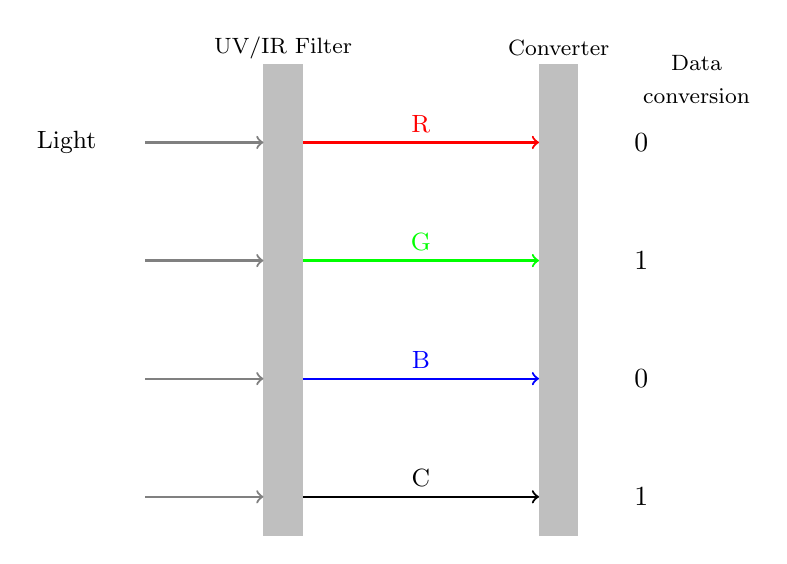
\begin{tikzpicture}
		
		% UV/IR Filter and Converter rectangles
		\fill[gray!50] (2, -2.5) rectangle (2.5, 3.5);
		\fill[gray!50] (5.5, -2.5) rectangle (6, 3.5);
		
		% Labels
		\node at (-0.5, 2.5) {\small Light};
		\node at (2.25, 3.7) {\footnotesize UV/IR Filter};
		\node at (5.75, 3.7) {\footnotesize Converter};
		\node[align=center] at (7.5, 3.3) {\footnotesize Data \\ \footnotesize conversion};
		
		% Arrows for light input
		\draw[->, thick, gray] (0.5, 2.5) -- (2, 2.5);
		\draw[->, thick, gray] (0.5, 1) -- (2, 1);
		\draw[->, thick, gray] (0.5, -0.5) -- (2, -0.5);
		\draw[->, thick, gray] (0.5, -2) -- (2, -2);
		
		% Color-coded arrows
		\draw[->, thick, red] (2.5, 2.5) -- (5.5, 2.5) node[midway, above] {\small R};
		\draw[->, thick, green] (2.5, 1) -- (5.5, 1) node[midway, above] {\small G};
		\draw[->, thick, blue] (2.5, -0.5) -- (5.5, -0.5) node[midway, above] {\small B};
		\draw[->, thick, black] (2.5, -2) -- (5.5, -2) node[midway, above] {\small C};
		
		% Data conversion outputs
		\node at (6.8, 2.5) {0};
		\node at (6.8, 1) {1};
		\node at (6.8, -0.5) {0};
		\node at (6.8, -2) {1};
	\end{tikzpicture}
	
	\captionof{figure}{Schematic of the main function of a color sensor}
	\label{fig:SchematicColorSensor}
\end{center}

The block diagram \ref{fig:FunctionalBlockDiagram} shows the processing flow of the APDS-9660 from light detection to communication via the I²C protocol with the Arduino. The individual steps are explained as follows:

\tikzstyle{block} = [rectangle, draw, minimum width=3.5cm, minimum height=1.2cm, text centered, text width=3.5cm]
\tikzstyle{smallblock} = [rectangle, draw, minimum width=3.5cm, minimum height=1.2cm, text centered]
\tikzstyle{arrow} = [thick,->,>=stealth]
\tikzstyle{sensor} = [draw, isosceles triangle, isosceles triangle apex angle=60, shape border rotate=-90, minimum height=1.5cm, minimum width=1.5cm, text centered]

\begin{center}
	\begin{tikzpicture}[node distance=2.5cm, scale=0.5, every node/.style={transform shape}]
		
		% Sensors
		\node (clear) [sensor] {Clear};
		\node (red) [sensor, below of=clear] {Red};
		\node (green) [sensor, below of=red] {Green};
		\node (blue) [sensor, below of=green] {Blue};
		
		% RGBC + ALS
		\node (rgbc_als) [block, right of=red, xshift=3cm] {RGBC \\ ALS};
		
		% MUX
		\node (mux) [smallblock, right of=rgbc_als, xshift=3cm] {MUX};
		
		% ADC
		\node (adc) [smallblock, right of=mux, xshift=3cm] {ADC};
		
		% FIFO + Threshold Control
		\node (fifo) [block, right of=adc, xshift=3.5cm] {32 x 4 Byte FIFO \\ Threshold Control};
		
		% I2C Interface
		\node (i2c) [block, above of=fifo, yshift=2cm] {I\textsuperscript{2}C Interface};
		
		% Interrupt
		\node (interrupt) [smallblock, below of=fifo, yshift=-2cm] {Interrupt};
		
		% Connections
		\draw [arrow] (clear) -- (rgbc_als);
		\draw [arrow] (red) -- (rgbc_als);
		\draw [arrow] (green) -- (rgbc_als);
		\draw [arrow] (blue) -- (rgbc_als);
		\draw [arrow] (rgbc_als) -- (mux);
		\draw [arrow] (mux) -- (adc);
		\draw [arrow] (adc) -- (fifo);
		\draw [arrow] (fifo) -- (i2c);
		\draw [arrow] (fifo) -- (interrupt);
		\draw [arrow] (i2c) -- ++(2.5cm,0) node[right] {SCL};
		\draw [arrow] (i2c) -- ++(2.5cm,-1.5cm) node[right] {SDA};
		\draw [arrow] (interrupt) -- ++(2.5cm,0) node[right] {INT};
		
	\end{tikzpicture}
	
	\captionof{figure}{Functional Block Diagram}
	\label{fig:FunctionalBlockDiagram}
\end{center}

\Mynote{The graphic is not optimal. Description of the individual blocks is not clear. What does RGBC and ALS mean?}


The photodiodes convert the intensities of the color components of the filtered light and the total light into electrical signals.
These RGBC (Red, Green, Blue, Clear) and ALS (Ambient Light Sensor) signals are forwarded to the next processing stage using the multiplexer (MUX). 

The MUX allows for the sequential processing of the color signals, as the ADC (Analog-to-Digital Converter) can only process one signal at a time.
The ADC converts the analog signal selected by the MUX into a digital value. This conversion is necessary to make the signal suitable for digital processing and transmission.

The digital value is stored in a FIFO (First In, First Out) data register, which can store up to 32 data values (4 bytes each). A threshold controller monitors the data and triggers an interrupt when defined limits are reached. The detailed process is explained in Chapter Data Processing \ref{chap:Data Processing}.

The stored data is transmitted to the Arduino via an I²C bus. The I²C bus uses two lines: the SCL (Serial Clock Line) for the clock and the SDA (Serial Data Line) for data transmission. The detailed functioning of the I²C bus is explained in Chapter \ref{chap:Protokoll I²C} Protokoll I²C.
\cite{Avago:2015}.

\subsubsection{Data Processing}
\label{chap:Data Processing}

The color detection begins at the photodiodes with RGBC detection and ends with 16-bit values stored in the RGBC data registers. The signal from the photodiode array is accumulated over a period defined by the value in the ATIME register (ALS ADC Integration Time) before the results are transferred to the RGBCDATA registers. The gain factor can be set from 1x to 64x, which is controlled via the CONTROL<AGAIN> bit (ALS Gain Control). Performance parameters such as accuracy, resolution, conversion speed, and energy consumption can be adjusted to meet the application requirements.

Between measurements, a customizable, energy-efficient waiting period is maintained, the duration of which is determined by the control bits WEN (Wait Enable), WTIME (Wait Time), and WLONG (Wait Long Enable). The waiting time can range from 0 seconds to a maximum of 8.54 seconds.

An interrupt is triggered when the clear channel values exceed the thresholds defined in the AILTL/AIHTL (ALS low threshold, lower byte/ALS high threshold, lower byte) or AILTH/AIHTH (ALS low threshold, upper byte/ALS high threshold, upper byte) threshold registers. To avoid unwanted or false interrupts, a persistence filter is integrated, ensuring that an interrupt is triggered only when a defined number of consecutive values fall outside the thresholds. This threshold is set in the APERS register (ALS Interrupt Persistence). If a value is within the thresholds, the persistence counter is reset. If the analog circuit is saturated, the ASAT bit is set, indicating potentially inaccurate RGBCDATA results. The AINT (ALS Interrupt) and CPSAT (Clear Diode Saturation) bits can be queried at any time via I²C. However, for AINT to trigger a hardware interrupt on the INT pin, the AIEN bit (ALS Interrupt Enable) must be set. Saturation of the analog-to-digital converter can be detected via the CPSAT bit; to enable this function, the CPSIEN bit (Clear Diode Saturation Interrupt Enable) must be set. The AVALID bit (ALS Valid) is reset by reading the RGBCDATA. ASAT and AINT can be reset via the CICLEAR (Clear Channel Interrupt Clear) or AICLEAR (All Non-Gesture Interrupt Clear) bits.

The RGBC results can be used to determine the color temperature in Kelvin or the ambient light intensity in Lux.

\cite{Avago:2015}








\section{Specific Sensor}

cite board

\section{Specification}

\begin{itemize}
  \item cite data sheet
  \item Circuit Diagram
\end{itemize}

\section{Bibliothek}

\subsection{Description}

\subsection{Installation}

\subsection{Functions}

\subsection{Example - Manual}

\subsection{Example}

\subsection{Example - Code}

\subsection{Example - Files}



\section{Calibration}

cite method

\section{Simple Code}


\section{Simple Application}



\section{Tests}

\subsection{Simple Function Test}

\subsection{Test all Functions}

\section{Simple Application}


\section{Further Readings}

